
% \graphicspath{{figure/maegaki}}
% かけ！！！！！！！！！！！！！！！！！！！！！！！！！！！！！！！！
% \\\\\textbf{〈IR2110〉（編集者兼著者兼イラスト担当）}
% % \\\hspace{5mm}\hrule height 0.1mm depth 0.1mm width \linewidth
% % ~\\\par
% \newpage
% 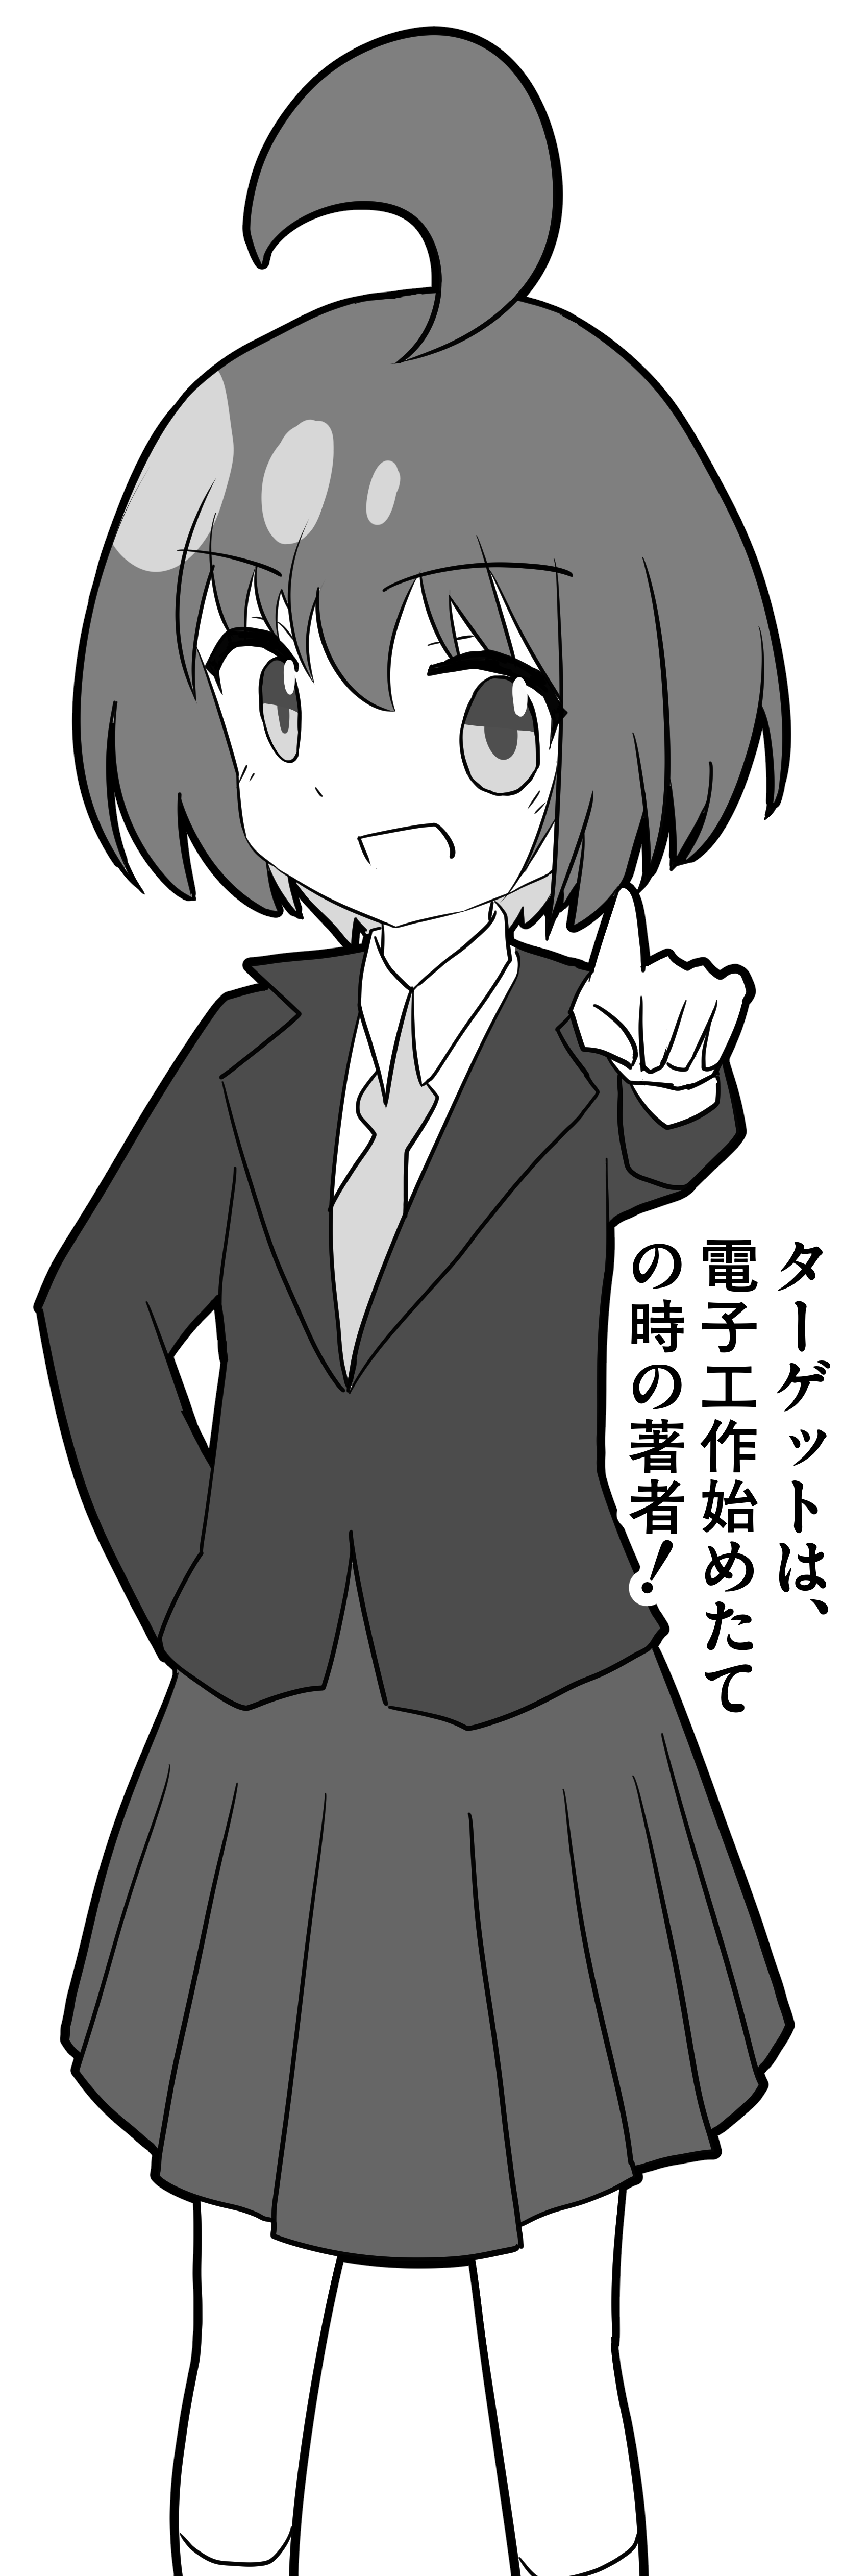
\includegraphics[width=72mm]{まえがき_2.png}
% \clearpage
{
    \renewtcolorbox{partbox}{
        boxrule=0mm,
        breakable,
        arc=0mm,colback=white,
        left=0mm,right=0mm,bottom=0mm,top=0mm,
        colframe=white
    }
    \renewtcolorbox{sectionbox}{
        notitle,colback=white,colframe=black,arc=0mm,
        sharp corners=all,bottomrule=0.25mm,
        toprule=-0.2mm,leftrule=-0.2mm,rightrule=-0.2mm,
        left=0mm,boxsep=0mm,enlarge bottom by = -3mm
    }

    % \RenewBlockHeading{section}{1}{
    % font=\fontsize{32\Q}{0mm}\shingothicB,
    % align=left,
    % label_format={},
    % subtitle_format={（#1）},
    % format={\jlreqHeadingLabel{#1}\jlreqHeadingText{#2} \vspace{2mm}\hrule height 0.1mm depth 0.1mm width \linewidth\begin{flushright}\normalsize\texttt{C　　O　　N　　T　　E　　N　　T　　S}\end{flushright}\vspace{6mm}},
    % subtitle_break=true
    % }

    \renewcommand{\section}[1]{
    }
    \renewcommand{\contentsname}{}

    \renewcommand{\thesubsection}{コラム\arabic{part}−\arabic{column}}
    {
        \onecolumn
        {
            \fontsize{32\Q}{0mm}\shingothicB\hspace{-1\zw}目次\vspace{2mm}\hrule height 0.1mm depth 0.1mm width \linewidth\begin{flushright}\normalsize\texttt{C　　O　　N　　T　　E　　N　　T　　S}\end{flushright} \vspace{2mm}
        }
        \bookmark[page=\thepage,level=1]{目次}
        \tableofcontents
    }
}
\twocolumn
\setcounter{part}{-1}